\section{Programming models}

\subsection{Implicit SPMD Program Compiler (ISPC)}

Before introducing the ISPC compiler, we give the definition of SPMD.

\begin{definitionbox}[: Single Program, Multiple Data (SPMD)]
    \definition{Single Program, Multiple Data (SPMD)} is a term that has been used to refer to computational models for exploiting parallelism, where \textbf{multiple processors work together to execute a program to achieve faster results}.

    The \textbf{difference} between \emph{SPMD} and \emph{SIMD} (page \pageref{subsubsection: Single Instruction, Multiple Data (SIMD) processor}) is that in SPMD parallel execution, \textbf{multiple autonomous processors simultaneously execute the same program at independent points}, rather than in SIMD it is vectorization at the instruction level so that \textbf{each CPU instruction processes multiple data elements}.

    In other words:
    \begin{itemize}
        \item SPMD: is the \textbf{programming abstraction}, because the programmer has to think; the program is written in terms of this abstraction.
        \item SIMD: in general, the compilers (ISPC) issue special vector instructions that execute the logic performed by each parallel instance created (ISPC gang spawned). In addition, the compilers handle the mapping of conditional control flow to vector instructions.
    \end{itemize}
    The difference and the terminology used by ISPC will become clearer in the following pages. We suggest that finish this section and come back here in a moment.
\end{definitionbox}

\begin{definitionbox}[: Implicit SPMD Program Compiler (ISPC)]
    \definition{Implicit SPMD Program Compiler (ISPC)} is a \textbf{compiler for a variant of the C programming language}, with extensions for \emph{Single Program, Multiple Data (SPMD)} programming. Under the SPMD model, the programmer writes a program that generally appears to be a regular serial program, though the execution model is actually that a number of program instances execute in parallel on the hardware. In other words, the \textbf{ISPC gives the programmer some API to do parallelization on the code; it also generates high quality SIMD code to increase performance}.
\end{definitionbox}

\noindent
The definition, implementation, and other details are explained in the official \href{https://github.com/ispc/ispc}{Intel GitHub repository}.

\newpage

\begin{flushleft}
    \textcolor{Green3}{\faIcon{question-circle} \textbf{How it works?}}
\end{flushleft}
Let us take a general main program; when we call an \texttt{ispc} function, it causes a \textbf{spawn of gang of ISPC program instances upon return, all instances have completed}. These \textbf{instances execute the same ISPC code simultaneously}, and \textbf{each instance has its own copy of local variables}. Take the following ISPC code as an example:
\begin{lstlisting}[language=c++, mathescape]
export void ispc_sinx(
    uniform int N, $\label{code: uniform}$
    uniform int terms,
    uniform float* x,
    uniform float* result
){
    // assume N % programCount = 0
    for (uniform int i=0; i<N; i+=programCount) { $\label{code: programCount}$
        int idx = i + programIndex; $\label{code: programIndex}$
        float value = x[idx];
        float numer = x[idx] * x[idx] * x[idx];
        uniform int denom = 6; // 3!
        uniform int sign = -1;
        for (uniform int j=1; j<=terms; j++) { 
            value += sign * numer / denom
            numer *= x[idx] * x[idx];
            denom *= (2*j+2) * (2*j+3);
            sign *= -1;
        }
        result[idx] = value;
    }
}
\end{lstlisting}
In the example, the \texttt{programCount} (row \ref{code: programCount}) and \texttt{programIndex} (row \ref{code: programIndex}) variables, \texttt{uniform} (row \ref{code: uniform}, and so on) data type tell us:
\begin{itemize}
    \item \texttt{programIndex} gives the index of the SIMD-lane being used for running each program instance (in other words, it's a varying \textbf{integer value that has value zero for the first program instance, and so forth}).
    
    \item \texttt{programCount} gives the \textbf{total number of instances in the \emph{gang}}.
    
    \item A variable that is declared with the \texttt{uniform} qualifier represents a \textbf{single value that is shared across the entire \emph{gang}}. 
\end{itemize}
Together, these can be used to uniquely map executing program instances to input data (\href{https://ispc.github.io/ispc.html#parallel-iteration-with-programindex-and-programcount}{programIndex and programCount}, \href{https://ispc.github.io/ispc.html#uniform-data}{uniform data type}).

\highspace
With the ISPC analogy, the \definition{SPMD programming model} should be clear:
\begin{enumerate}
    \item \textbf{Single thread of control} (typically a main program);
    \item \textbf{Invoke} the \textbf{SPMD function} (in the previous example, the \texttt{ispc\_sinx} function);
    \item \textbf{SPMD execution}, then \textbf{multiple instances of the function run in parallel} (multiple logical threads of control);
    \item \textbf{Returns} and \textbf{resumes a single thread} of control.
\end{enumerate}

\newpage

\begin{figure}[!htp]
    \centering
    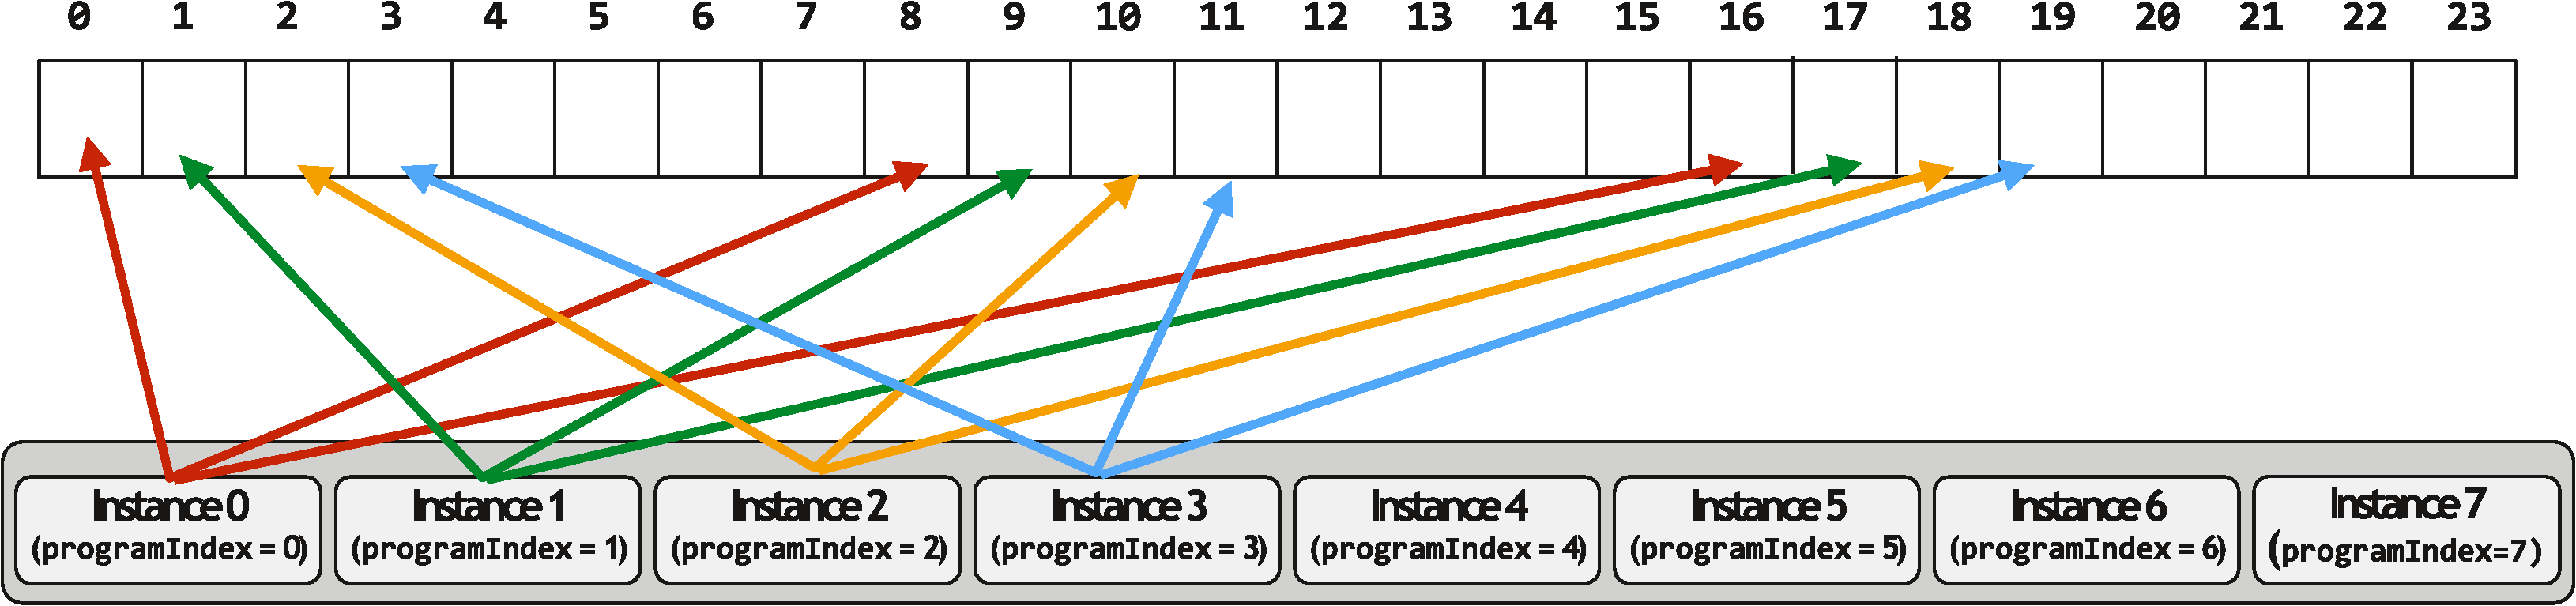
\includegraphics[width=\textwidth]{img/ispc-1.pdf}
    \begin{center}
        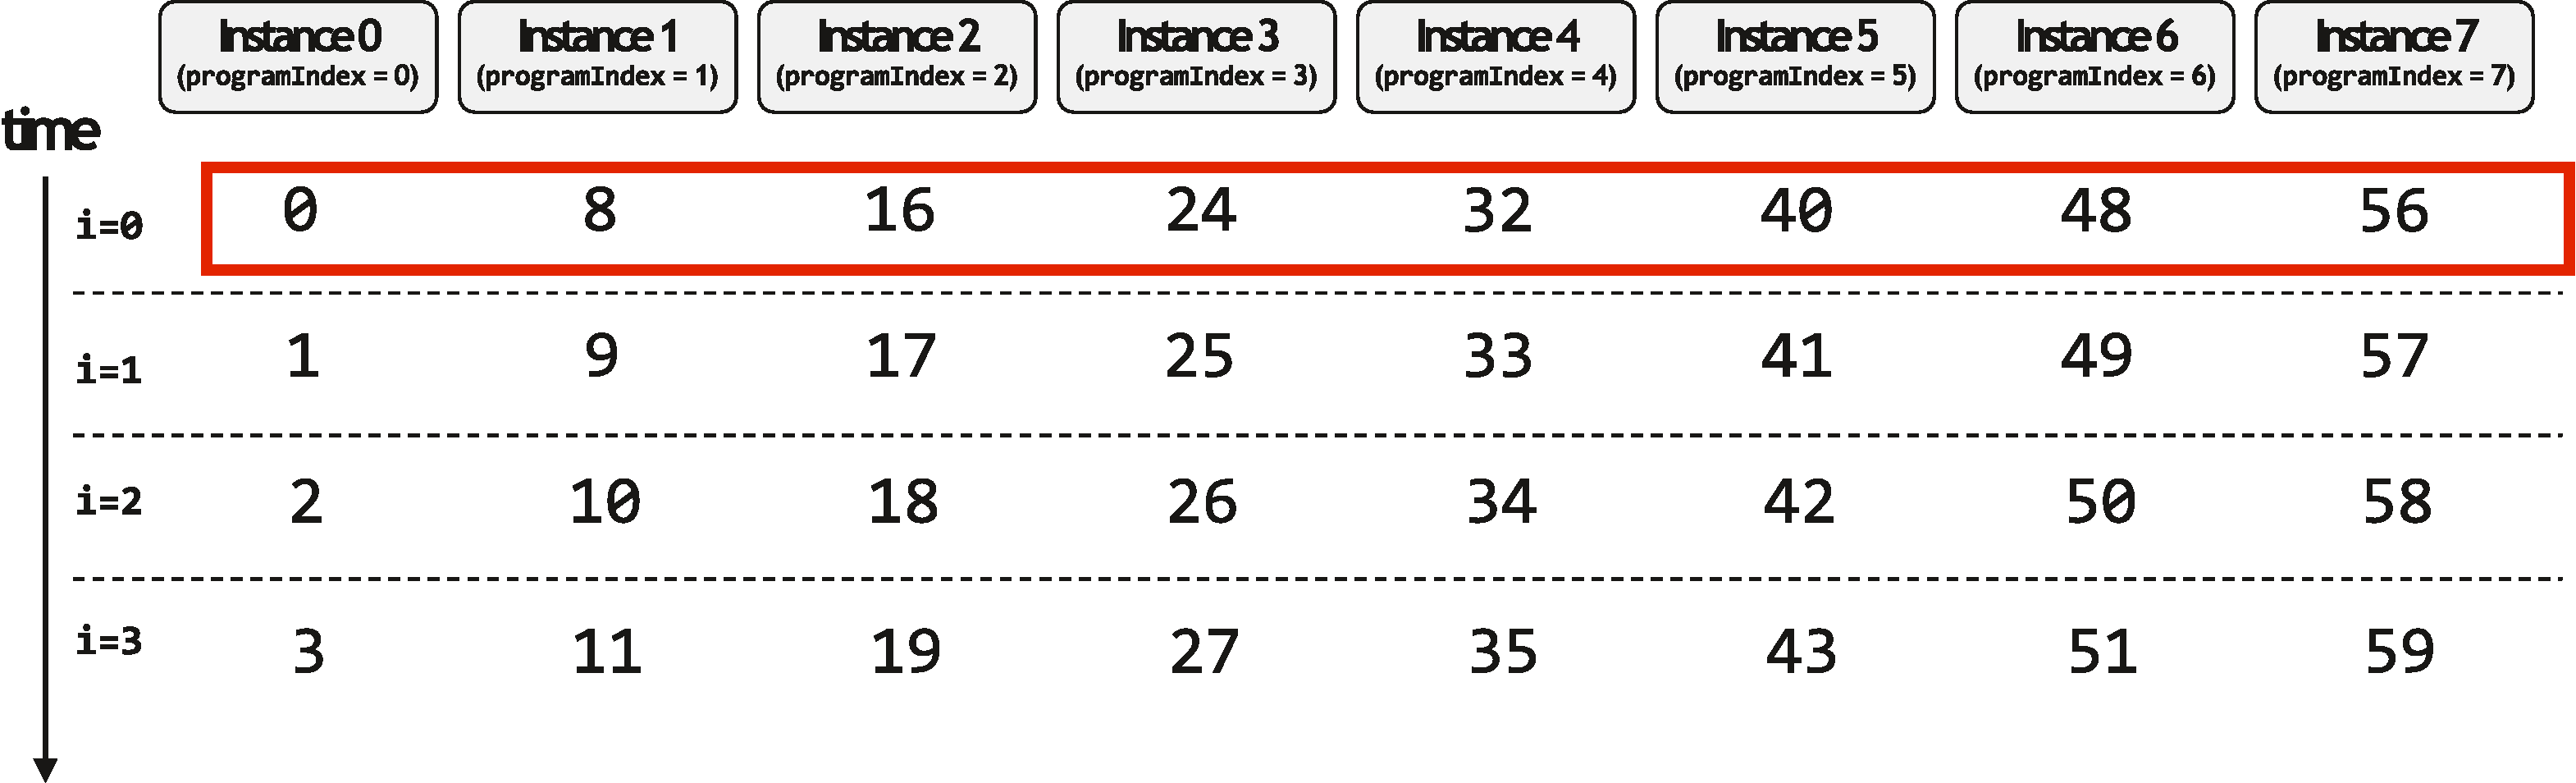
\includegraphics[width=\textwidth]{img/ispc-2.pdf}
    \end{center}
    \caption{Example of execution with 8 instances (\texttt{programCount} equal to 8). For all program instances, there are eight non-contiguous values in memory. A special instruction called \texttt{gather} is needed to implement this, but unfortunately it is a more complex and expensive SIMD instruction rather than a contiguous implementation.}
    \label{fig: ispc 8 instances, no optimized}
\end{figure}

\noindent
Figure \ref{fig: ispc 8 instances, no optimized} shows a possible execution of the ISPC function using 8 instances. The result is obtained and all is well. But there is one interesting observation. \textbf{Each ISPC instance writes each value in a non-contiguous way}. This can be done better:
\begin{lstlisting}[language=c++, mathescape]
export void ispc_sinx_v2(
    uniform int N,
    uniform int terms,
    uniform float* x,
    uniform float* result
){
    // assume N % programCount = 0
    uniform int count = N / programCount;
    int start = programIndex * count;
    for (uniform int i=0; i<count; i++) {
        int idx = start + i;
        float value = x[idx];
        float numer = x[idx] * x[idx] * x[idx];
        uniform int denom = 6; // 3!
        uniform int sign = -1;
        for (uniform int j=1; j<=terms; j++) { 
            value += sign * numer / denom
            numer *= x[idx] * x[idx];
            denom *= (j+3) * (j+4);
            sign *= -1;
        }
        result[idx] = value;
    }
}
\end{lstlisting}
\newpage
\begin{figure}[!htp]
    \centering
    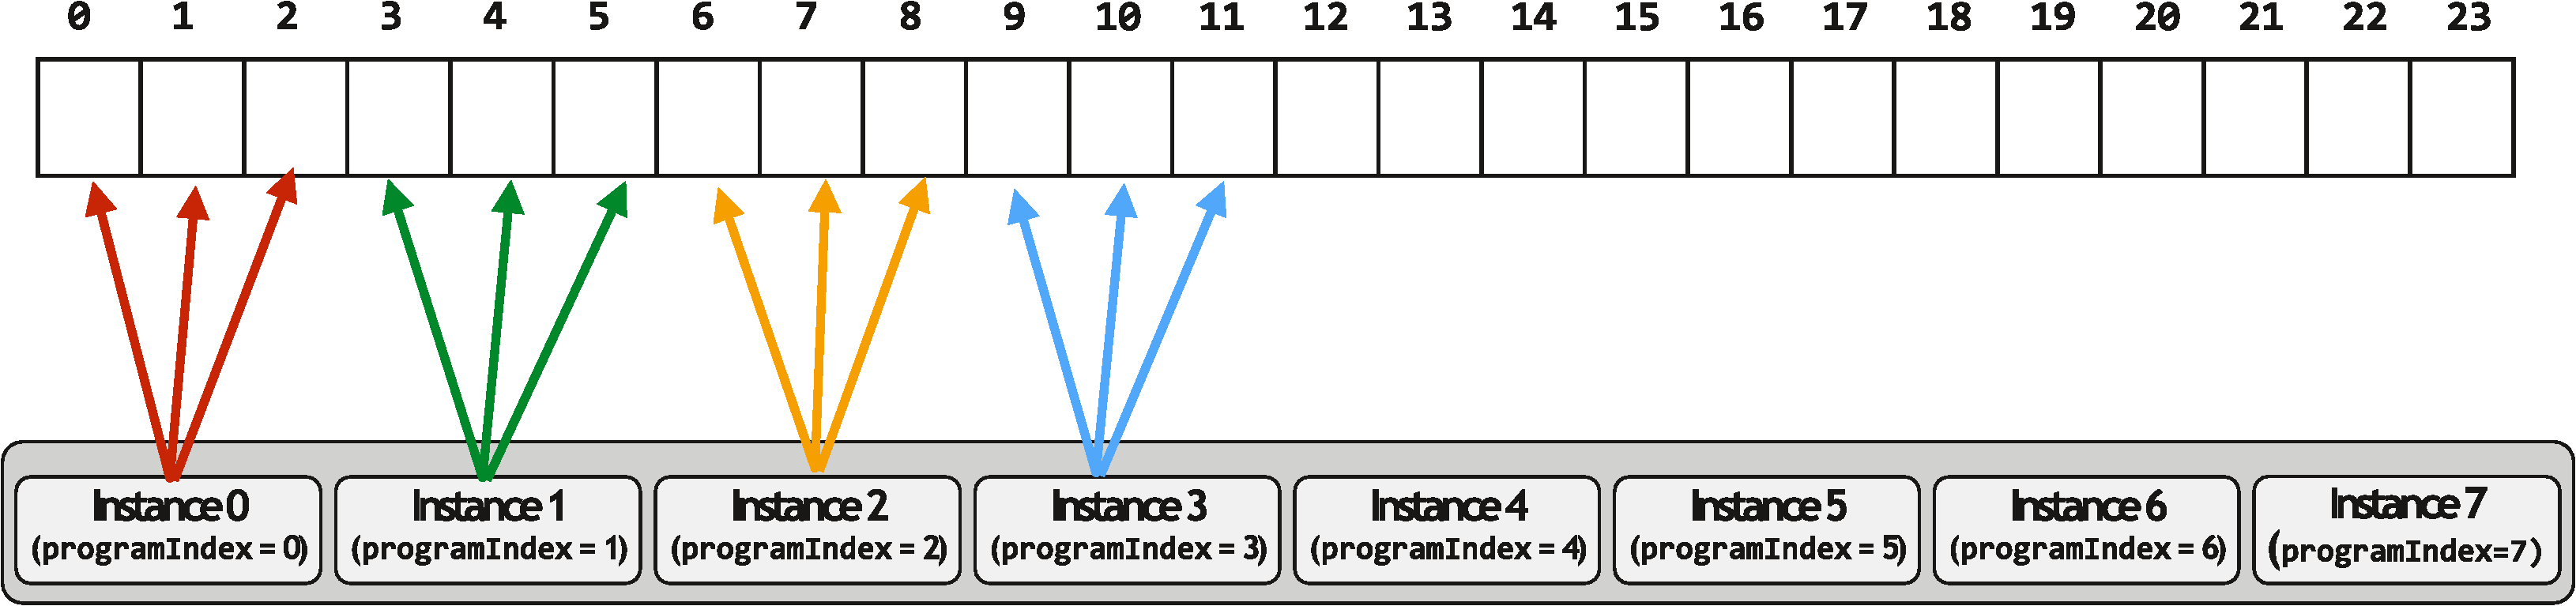
\includegraphics[width=\textwidth]{img/ispc-3.pdf}
    \begin{center}
        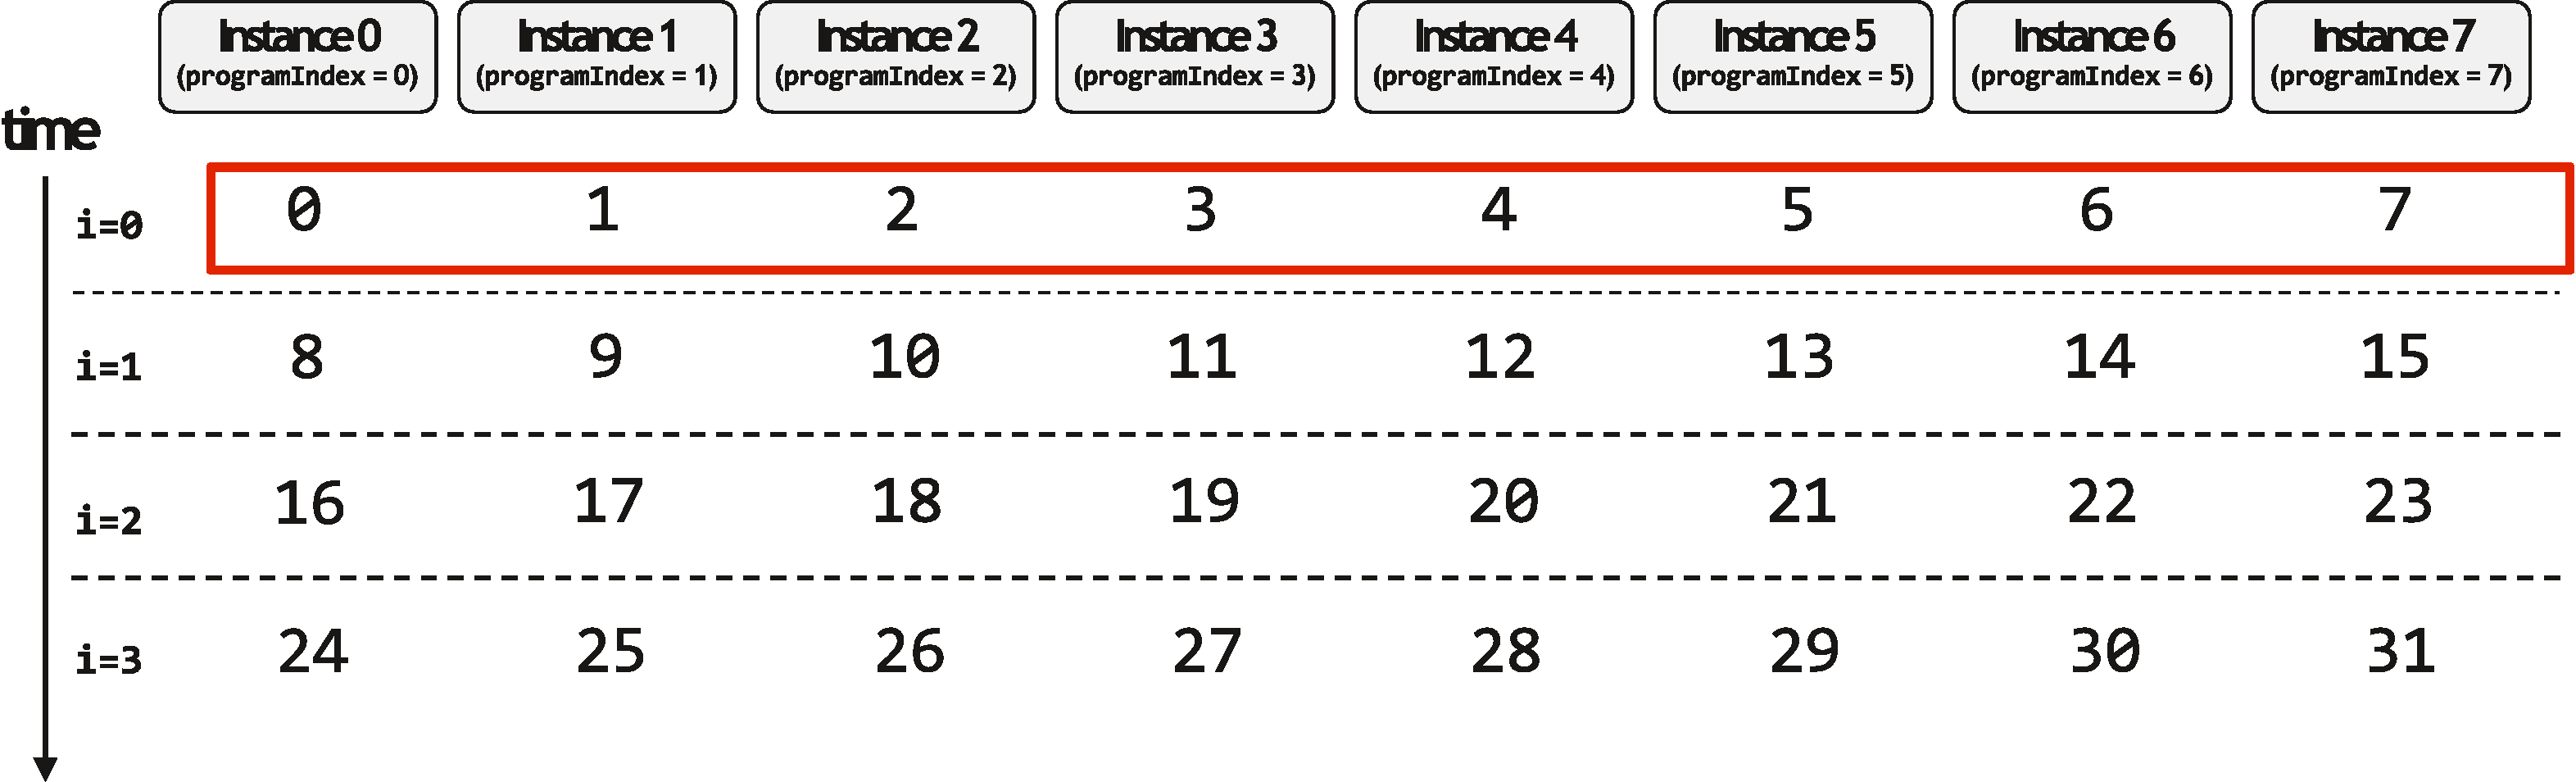
\includegraphics[width=\textwidth]{img/ispc-4.pdf}
    \end{center}
    \caption{Example of execution with 8 instances (\texttt{programCount} equal to 8). A single \dquotes{packed vector load} instruction efficiently implements this. For all program instances, since the eight values are contiguous in memory.}
\end{figure}